\subsection*{Question 3}

\textbf{a)} Using a \textbf{Metropolis algorithm} (\textit{with componentwise proposals}) and the R software (without using JAGS or other specific packages), draw a random sample from the posterior distribution of $(\vec{\theta}|\mathcal{D}_1)$.

\begin{center}\rule{6cm}{0.4pt}\end{center}

\inputminted[breaklines]{r}{code/q3a.r}

For the single component metropolis algorithm, we should aim for $\approx \SI{40}{\percent}$ of acceptance rate. We ran the algorithm for $\num{140000}$ steps and a burnin of $\num{5000}$ steps. In order to have such an acceptance rate for each $\theta$ parameter, we tweaked the sigma proposals to finally start with $\sigma = (0.017, 0.021, 0.019)$ giving us an acceptance rate of $(\SI{40}{\percent}, \SI{40}{\percent}, \SI{40}{\percent})$ respectively for $(\theta_0, \theta_1, \theta_2)$.

\begin{figure}[H]
	\centering
	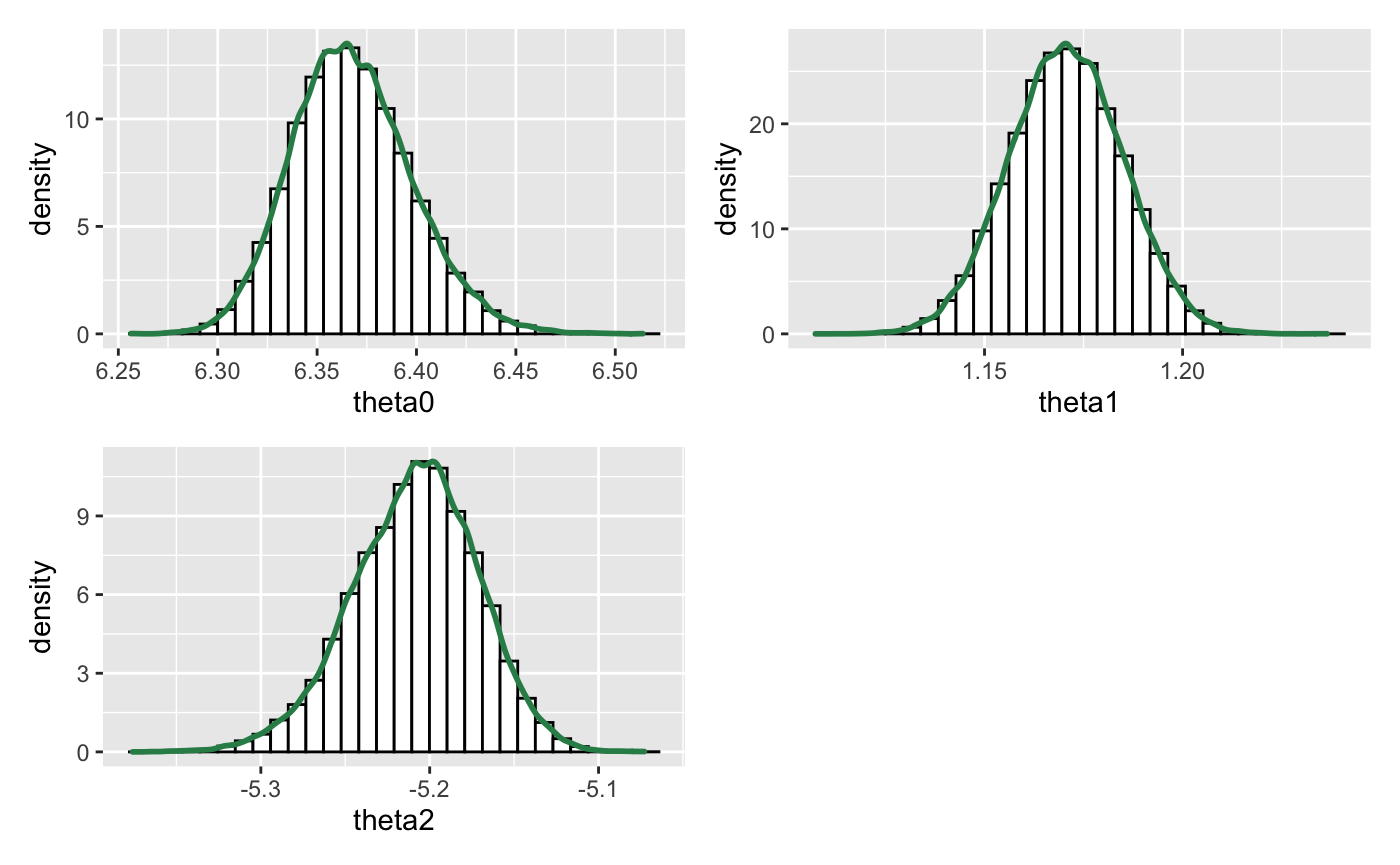
\includegraphics{figures/metropolis_cw/metropolis_cw_samples.png}
	\caption{Random sample from the posterior distribution of $(\vec{\theta}|\mathcal{D}_1)$ using a component-wise metropolis algorithm}
	\label{fig:metropolis_cw_samples}
\end{figure}

\textbf{b)} Evaluate the convergence of your algorithm. After a suitable burnin, evaluate the effective sample size for each $\theta_k$ and make sure that each of these values is at least $500$.

\begin{center}\rule{6cm}{0.4pt}\end{center}

Since there does not exist any statistical test that would be a proof of convergence, we will perform multiple tests or analysis in order to increase our confidence in the fact that our algorithm has effectively converged.

\subsubsection*{Visual analysis}

We can first perform a visual analysis to check for the convergence of the metropolis algorithm.

\begin{figure}[H]
	\centering
	\begin{subfigure}{0.3\textwidth}
		\centering
		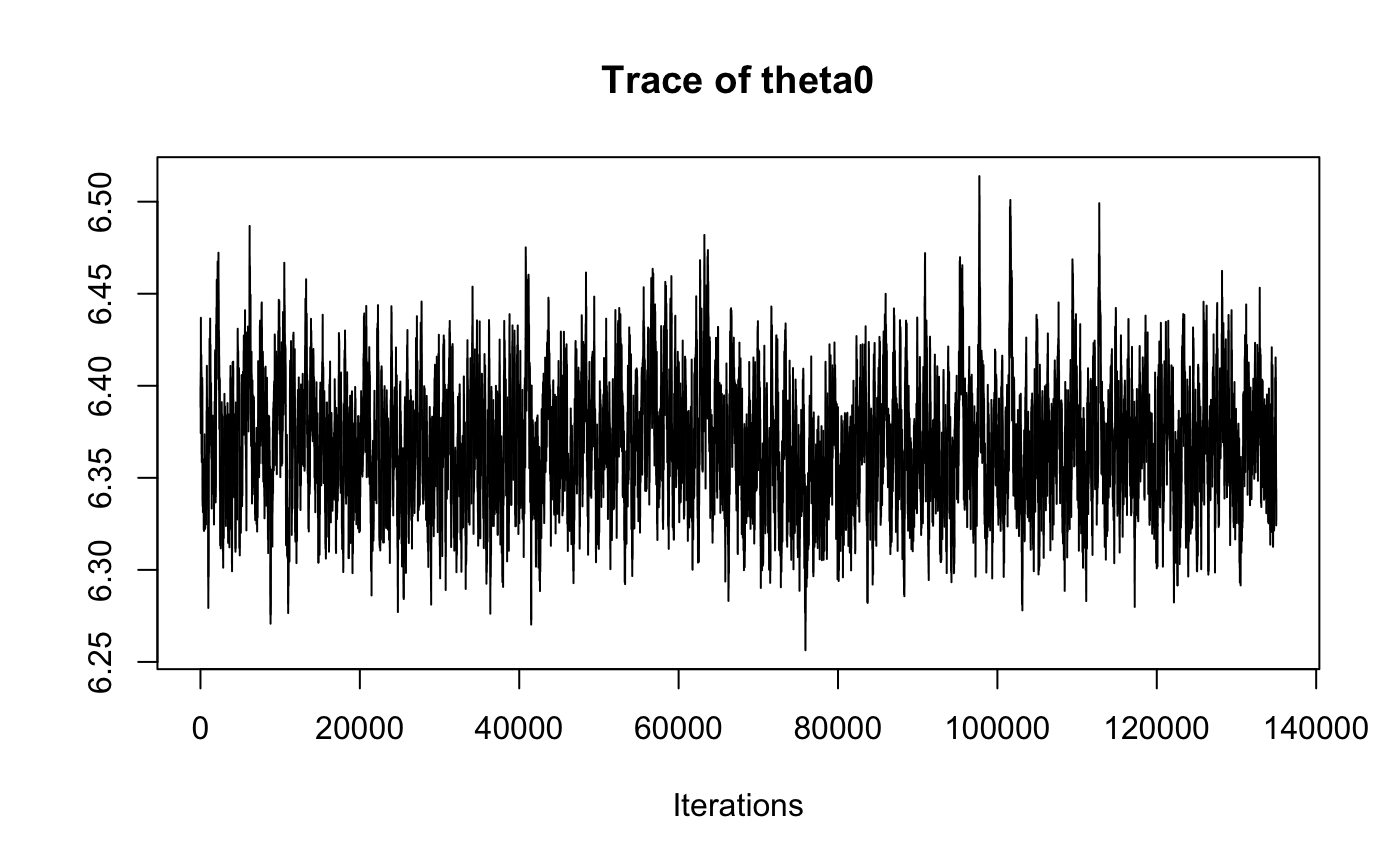
\includegraphics{figures/metropolis_cw/metropolis_cw_traceplot_theta0}
	\end{subfigure}
	\begin{subfigure}{0.3\textwidth}
		\centering
		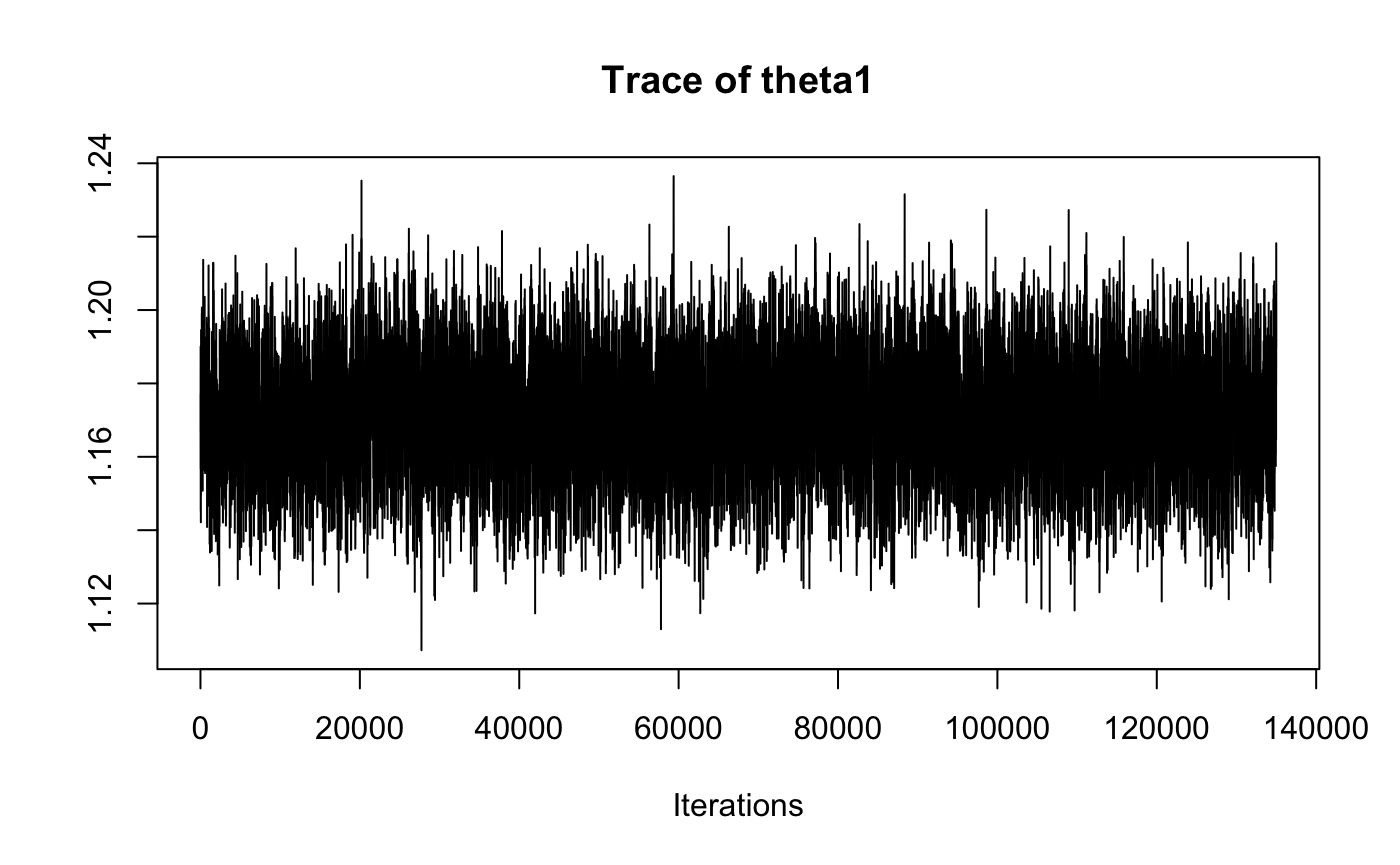
\includegraphics{figures/metropolis_cw/metropolis_cw_traceplot_theta1}
	\end{subfigure}
	\begin{subfigure}{0.3\textwidth}
		\centering
		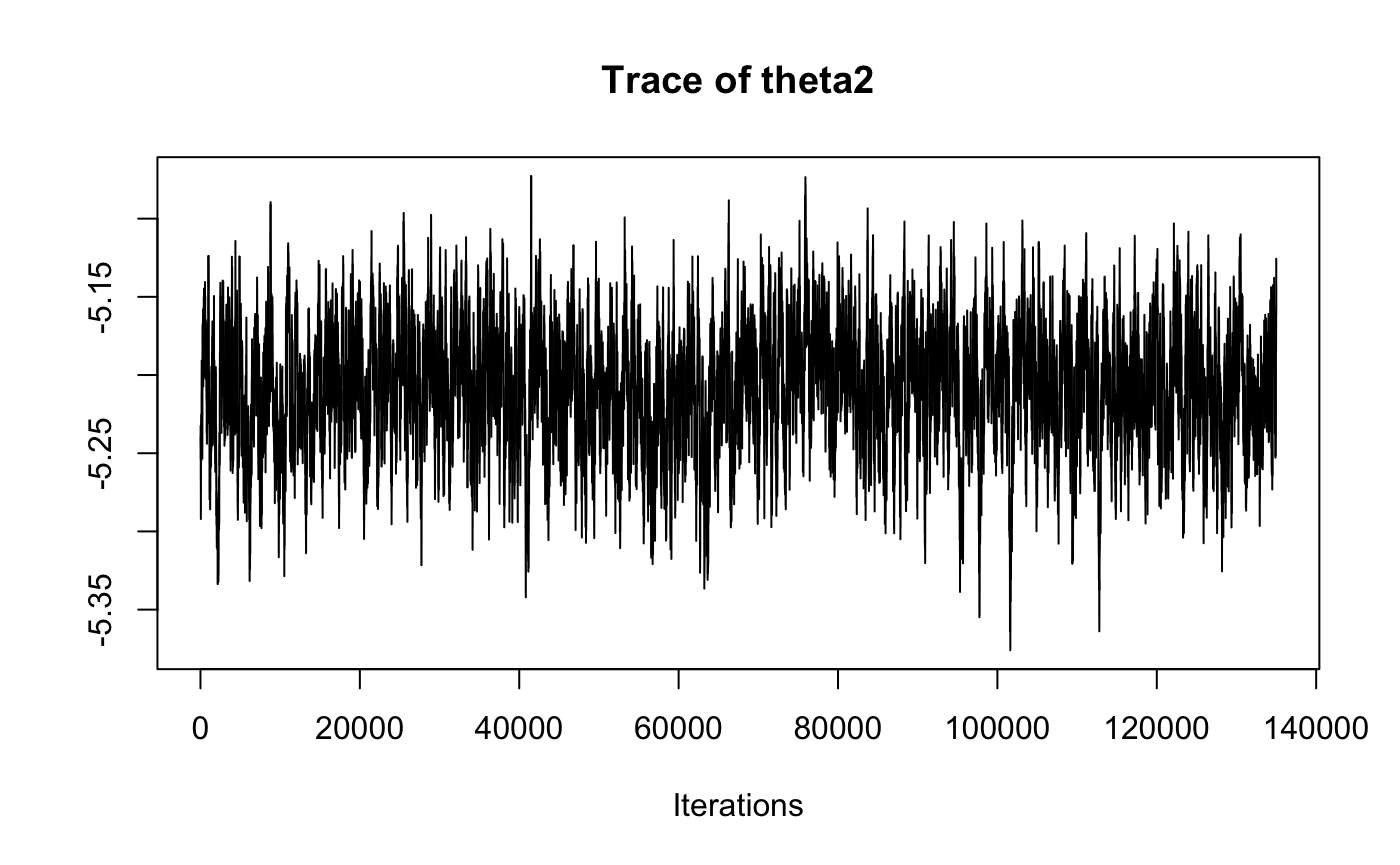
\includegraphics{figures/metropolis_cw/metropolis_cw_traceplot_theta2}
	\end{subfigure}
	\caption{Traceplots of the $\theta_k$ parameters}
	\label{fig:metropolis-cw-traceplots}
\end{figure}

The mixing is good for all the parameters and in particular for $\theta_1$. However, we can go further and use some statistical tools to increase our confidence in the convergence of these samples.

\subsubsection*{Gelman-Rubin statistic}

Imagine we would start multiple chains in parallel with different starting values. Then they all should converge to the stationnary distribution so that after some amount of time, one could not distinguish between the different chains. We can assess such a thing by comparing the variation between chains. If all chains converge toward the stationnary distribution, they all should be the same and therefore the variation between chains should be zero. This can be assessed with the Gelman-Rubin statistic.

Let $\bm{\theta_1},\dots,\bm{\theta_l}$ be different samples from Markov chains run in parallel with different initial values. As the length of the chains approaches infinity and the between chains variance approaches zero, the Gelman-Rubin statistic ($\hat{R}$) approaches the value of $1$. Practically, we can aim for a value of $\hat{R}$ in the neighborhood of $1.1$.

Here, we created three chains using different initial parameters for $\bm{\theta}$. The $\hat{R}$ of each parameter is almost equal to $1.0$ with an upper confidence interval below $1.1$.

\begin{table}[H]
	\centering\begin{tabular}{|c|c|c|} \hline 
		parameters & $\hat{R}$ & upper C.I. \\ \hline
		$\theta_0$ & $1.001888$ & $1.006282$ \\
		$\theta_1$ & $1.000398$ & $1.001150$ \\
		$\theta_2$ & $1.002163$ & $1.006658$ \\ \hline
	\end{tabular}
	\caption{Results of the Gelbman-Rubin test}
	\label{tab:metropolis-cw-gelman-rubin}
\end{table}

Moreover, we can notice below that the convergence appears after roughly $5000$ iterations for each parameter.

\begin{figure}[H]
	\centering
	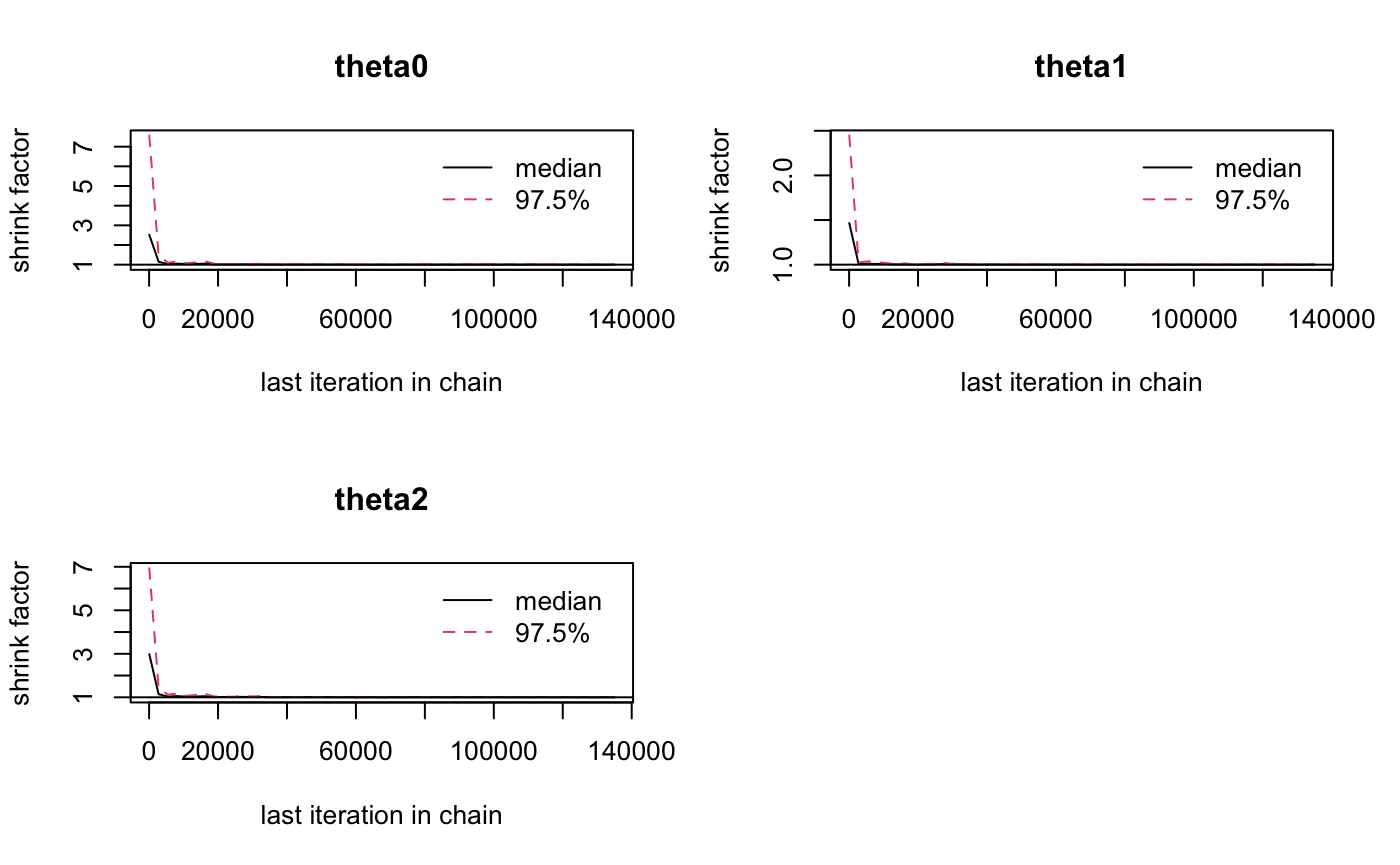
\includegraphics{figures/metropolis_cw/metropolis_cw_gelman-plot.png}
	\caption{Evolution of the Gelman-Rubin shrink factor with the number of iterations of the metropolis algorithm (component-wise)}
	\label{<label>}
\end{figure}

\subsubsection*{Geweke statistic}

The Geweke statistic has the particularity to assess convergence from a single chain. This statistic will perform a two mean test comparing the mean of the first $\SI{10}{\percent}$ of the chain with the last $\SI{50}{\percent}$. If convergence has occured, the two means should be equal. Practically, we use a classical z-score test from frequentist statistic based on the effective sample sizes.

\begin{table}[H]
	\centering\begin{tabular}{|c|c|c|} \hline 
		parameters & z-score & p-value \\ \hline
		$\theta_0$ & $-1.3259$ & $0.9075636$ \\
		$\theta_1$ & $-0.5802$ & $0.7191101$ \\
		$\theta_2$ & $1.1019$ &  $0.1352526$ \\ \hline
	\end{tabular}
	\caption{Results for the Geweke statistic (z-score)}
	\label{tab:metropolis-cw-geweke}
\end{table}

We notice that at a $\SI{5}{\percent}$ significance level, one cannot reject the hypothesis that the means of the two subchains are equal the z-score. To conclude, none of these statistcs showed us that our algorithm did not converge into the stationnary distribution. We can be confident and go further.

% \begin{figure}[H]
% 	\centering
% 	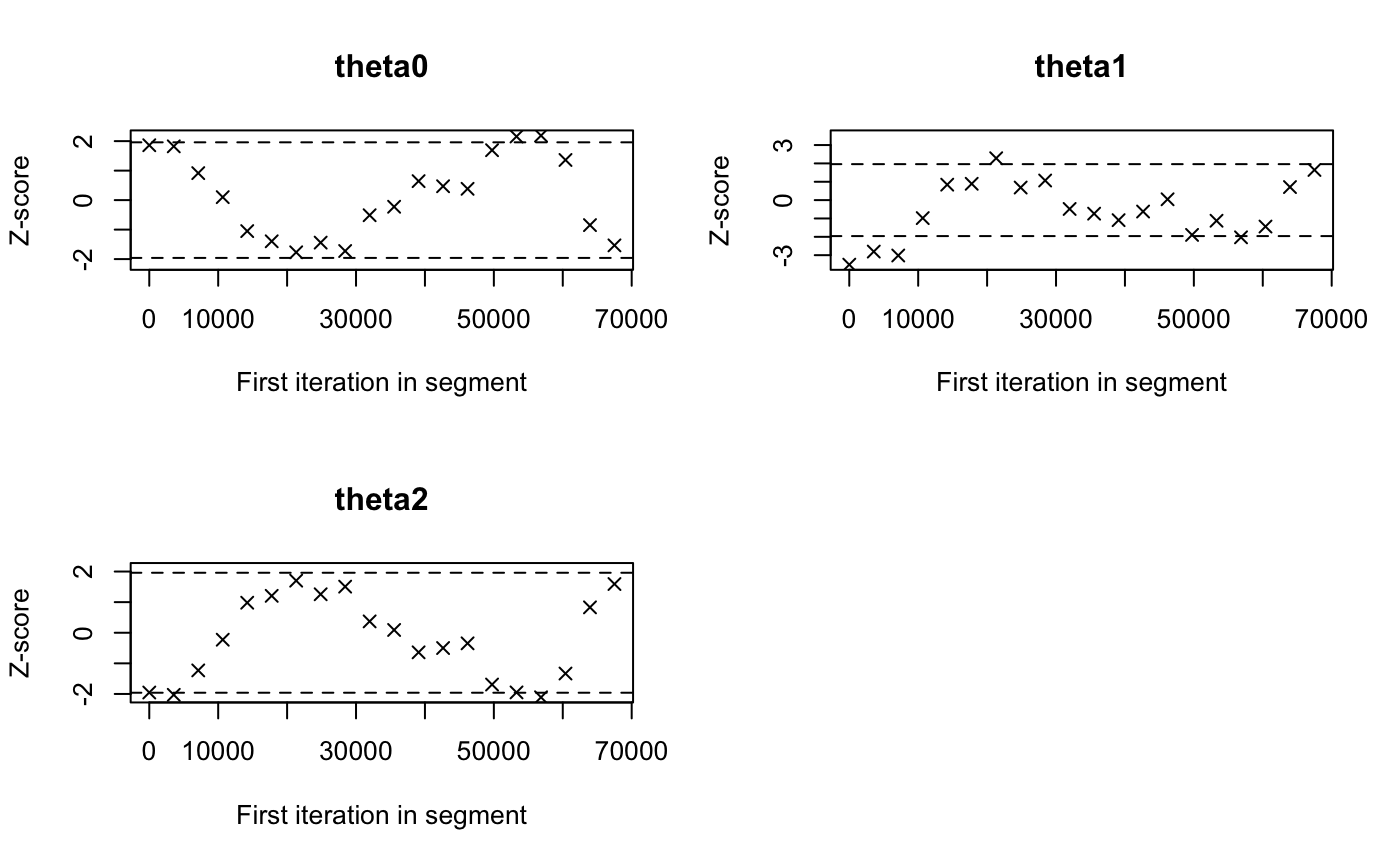
\includegraphics{figures/metropolis_cw_geweke-plot.png}
% 	\caption{Evolution of the Gelman-Rubin Z-score with the number of iterations of the metropolis algorithm (component-wise)}
% 	\label{fig:metropolis-cw-geweke-plot}
% \end{figure}

\subsubsection*{Effective sample sizes}

Computing the effective sample size (\textit{i.e. the number of samples that would be generated if there were no autocorrelation}) for each parameter after a burnin of $5000$ iterations, we can confirm that we have at least $500$ samples for each $\theta_k$.

\begin{table}[H]
	\centering\begin{tabular}{|c|c|c|} \hline 
		$\theta_0$ & $\theta_1$ & $\theta_2$ \\ \hline 
		$683.7875$  & $4121.8599$ & $648.4315$   \\ \hline
	\end{tabular}
	\caption{Effective sample sizes}
	\label{tab:metropolis-cw-effective-sample-sizes}
\end{table}

\textbf{c)} Compare the observed count data series for experiment $1$ with the fitted curve for $\mu(t)$

\begin{center}\rule{6cm}{0.4pt}\end{center}

\begin{figure}[H]
	\centering
	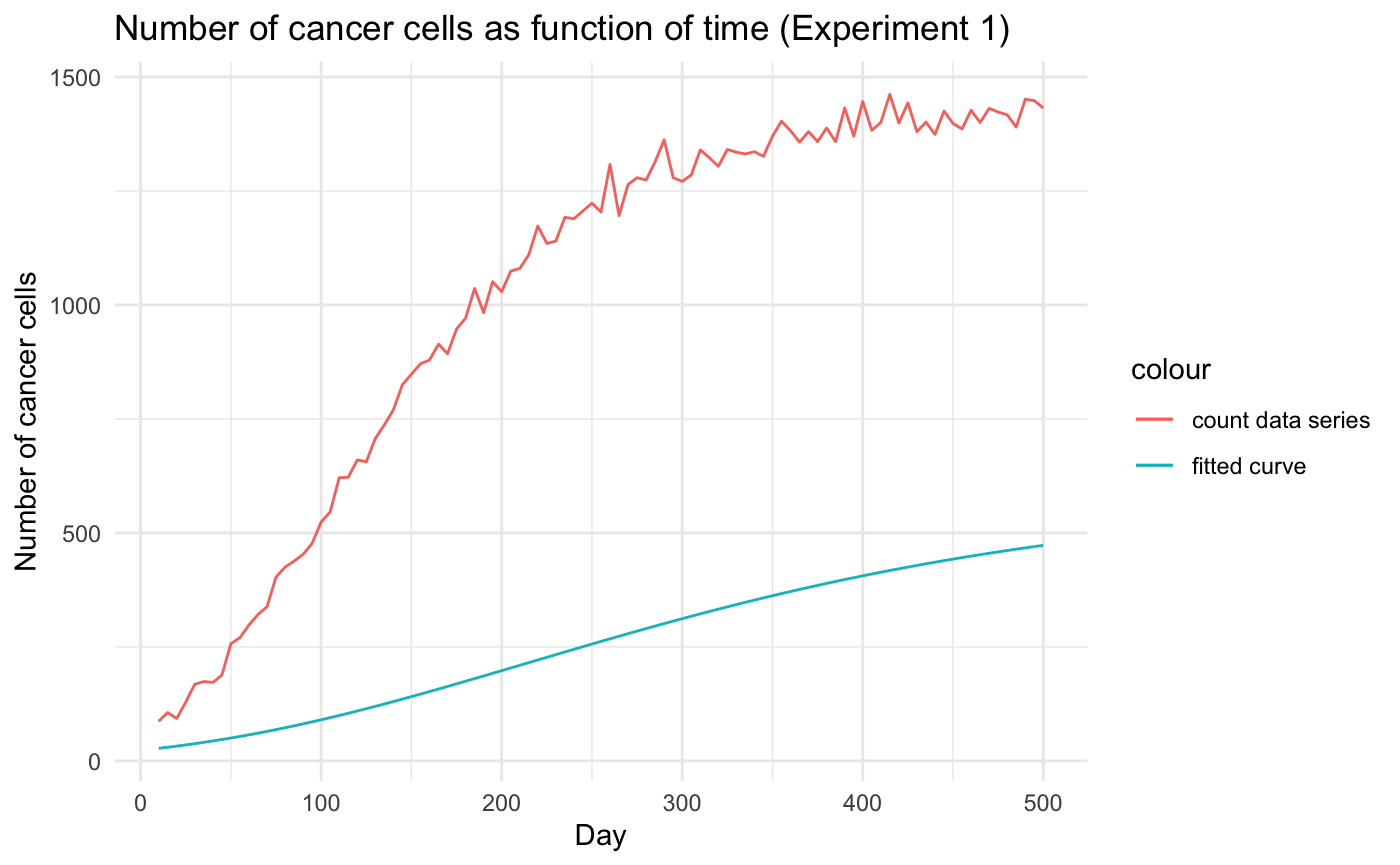
\includegraphics[width=0.7\textwidth]{figures/metropolis_cw/metropolis_cw_fitted_curve.png}
	\caption{Comparison of the observed count data series for experiment 1 (\textit{black}) with the fitted curve for $\mu(t)$ (\textit{red})}
	\label{fig:metropolis-cv-fitted-curve}
\end{figure}

On the plot above, it seems like the fitted curve for $\mu(t)$ computed with the mean parameters of $\bm{\theta}$ --- that were obtained with the component-wise metropolis algorithm ran for the first experiment --- underestimate a lot the growth of the number of cancer cells as function of time.

\textbf{d)} Provide point estimates and $\SI{95}{\percent}$ credible regions for $\beta_0$, $\beta_1$, $\beta_2$.

\begin{center}\rule{6cm}{0.4pt}\end{center}

Using the relations found in the first question, we can find the estimations for the $\bm{\beta}$ parameters. We can then compute the mean and median of the $\bm{\theta}$ parameters as well as their respective $\SI{95}{\percent}$ credible regions.   The results are summarized in the tables below.

\begin{table}[H]
	\parbox{0.45\linewidth}{
		\centering
		\begin{tabular}{|c|c|c|} \hline 
			Parameter & Median & Mean \\ \hline 
			$\beta_0$ & $23.25$ & $23.28$ \\ 
			$\beta_1$ & $0.02$ & $0.02$ \\
			$\beta_2$ & $\num{5.46e-3}$ & $\num{5.46e-3}$ \\ \hline
		\end{tabular}
		\caption{Point estimates of $\bm{\beta}$}
		\label{tab:metropolis-cw-point-estimates}
	}
	\hfill
	\parbox{0.45\linewidth}{
		\centering
		\begin{tabular}{|c|c|c|} \hline 
			Parameter & Lower & Upper \\ \hline 
			$\beta_0$ & $20.5347$ & $26.0316$ \\ 
			$\beta_1$ & $0.0160$ & $0.0191$ \\
			$\beta_2$ & $0.0050$ & $0.0058$ \\ \hline
		\end{tabular}
		\caption{$\SI{95}{\percent}$ credible region for $\bm{\beta}$}
		\label{tab:metropolis-cw-credible-region}
	}
\end{table}

\textbf{e)} Provide a point estimates and $\SI{95}{\percent}$ credible region for the expected number of cancer cells at time $t = 0$ and $t = +\infty$ for experiment $1$.